\begin{esercizio}
   An electron is under the action of a constant magnetic field $\vb{B}=B_z(0,0,1)$. At $t=0$ a magnetic field along the $\hat{x}$ direction is turned on; its strength increases uniformly from $0$ to $B_x$ at time $t=T$ and then remains constant. The electron is initially in the spin-up state. Assume $B_x \ll B_z$.
   \begin{enumerate}[label=\alph*), leftmargin=0.6cm]
      \item Find the transition amplitude to the spin-down state at $t=T$ in the first order of perturbation theory.
      \item Calculate with a good approximation the transition probability for $B_z=5 \cdot 10^6 \rm \; V/m$, $B_x=10^5 \rm \; V/m$ and $T=\frac{mc}{e B_x}$. Is perturbation theory valid?
      \item Calculate in eV the first nonzero correction to the energy levels for $t \gg T$.
   \end{enumerate}
\end{esercizio}
\begin{soluzione}
   Sappiamo che, in generale, l'hamiltoniana di una particella in un campo magnetico è
   \begin{equation*}
      H=-\vb*{\mu} \vdot \vb{B}
   \end{equation*}
   dove $\vb*{\mu}$ è il momento magnetico della particella. Nel caso di un elettrone, il momento magnetico è dato da
   \begin{equation*}
      \vb*{\mu}
      =\frac{\hbar e}{2 m c} \vb*{\sigma}
   \end{equation*}
   dove $\vb*{\sigma}$ sono le matrici di Pauli.\\
   Analizziamo adesso il problema. Inizialmente abbiamo l'azione di un campo magnetico costante diretto lungo $\hat{z}$, dunque l'hamiltoniana assume la forma
   \begin{equation*}
      H_0=-\frac{\hbar e}{2 m c} B_z \sigma_z
   \end{equation*}
   Ricordiamo che la matrice di Pauli $\sigma_z$ è definita come
   \begin{equation*}
      \sigma_z
      =
      \begin{pmatrix}
         1 & 0 \\
         0 & -1
      \end{pmatrix}
   \end{equation*}
   e dunque i livelli energetici sono
   \begin{equation*}
      E_{\uparrow}=\frac{\hbar e B_z}{2 m c}
      \qq{e}
      E_{\downarrow}=-\frac{\hbar e B_z}{2 m c}
   \end{equation*}
   Osserviamo che il ground state è quello con spin down, dunque $E_0=E_{\downarrow}$, mentre il primo stato eccitato è quello con spin up, dunque $E_1=E_{\uparrow}$. Inoltre tra i due stati c'è uno splitting in energia pari a $\Delta E=\frac{\hbar e B_z}{mc}$.\\
   Questa è la situazione prima del tempo $t=0$; una volta raggiunto tale istante viene accesso un campo magnetico che varia linearmente, dunque nella forma $B(t)=mt + q$. In particolare, sappiamo che $B_x(0)=0 \equiv q$ e $B_x(T)=B_x$, per cui il coefficiente angolare è dato da $m=B_x/T$. In definitiva l'espressione generale di tale campo è
   \begin{equation*}
      B(t)=\frac{B_x}{T}t
   \end{equation*}
   Possiamo adesso svolgere il punto a). Poiché tale campo dipende dal tempo, ci troviamo nel caso di teoria perturbativa dipendente dal tempo e dobbiamo calcolare l'ampiezza di transizione dovuta a questo campo magnetico. L'ampiezza di transizione dallo stato iniziale $\ket*{i}=\ket*{\uparrow}$ allo stato finale $\ket*{f}=\ket*{\downarrow}$ sarà
   \begin{equation}
      c_{i \to f}(T)
      =-\frac{i}{\hbar} \int_{0}^{T} \dd{t} e^{i \omega_{f,i} t} \, V_{f,i}
      \label{eq:ampiezza_di_transizione_al_tempo_T}
   \end{equation}
   dove
   \begin{equation}
      \omega_{f,i}
      =\frac{E_{\downarrow} - E_{\uparrow}}{\hbar}
      =-\frac{e B_z}{m c}
      \label{eq:omega_f_i_campo_magnetico}
   \end{equation}
   e $V_{f,i}=\mel*{\downarrow}{V(t)}{\uparrow}$. Calcoliamo tale elemento di matrice: dato che il potenziale che dobbiamo considerare è quello associato al campo magnetico lungo $x$, si ha
   \begin{equation*}
      V_{f,i}
      =\mel*{\downarrow}{\frac{\hbar e}{2 m c} \sigma_x B_x \frac{t}{T}}{\uparrow}
      =\frac{\hbar e}{2 m c} B_x \frac{t}{T}\mel*{\downarrow}{\sigma_x}{\uparrow}
   \end{equation*}
   Ricordiamo che $\sigma_x$ è definita come
   \begin{equation*}
      \sigma_x=
      \begin{pmatrix}
         0 & 1 \\
         1 & 0
      \end{pmatrix}
   \end{equation*}
   pertanto la sua azione è quella di scambiare gli stati up e down tra loro, per cui si ha che $\sigma_x \ket*{\uparrow}=\ket*{\downarrow}$ e quindi
   \begin{equation}
      V_{f,i}
      =\frac{\hbar e}{2 m c} B_x \frac{t}{T}
      \label{eq:elemento_di_matrice_campo_magnetico_variabile}
   \end{equation}
   in quanto $\braket*{\downarrow}=1$.\\
   Sostituendo la \eqref{eq:omega_f_i_campo_magnetico} e la \eqref{eq:elemento_di_matrice_campo_magnetico_variabile} nella \eqref{eq:ampiezza_di_transizione_al_tempo_T} otteniamo
   \begin{equation*}
      c_{i \to f}(T)
      =-\frac{i}{\hbar} \int_{0}^{T} \dd{t} e^{-i \frac{e B_z}{m c} t } \frac{\hbar e}{2 m c} B_x \frac{t}{T}
      =-i \frac{e B_x}{2 m c T} \int_{0}^{T} \dd{t} e^{-i \frac{e B_z}{m c} t } t
   \end{equation*}
   Ricordiamo che in generale si ha
   \begin{equation*}
      \int_{0}^{T} \dd{t} e^{- a t} t
      =\left. -\frac{1}{a} e^{-a t} t \right|_{0}^{T} + \frac{1}{a} \int_{0}^{T} \dd{t} e^{-a t}
      =-\frac{1}{a} e^{-a T} T - \frac{1}{a^2} \qty( e^{-a T} - 1 )
   \end{equation*}
   Nel nostro caso $a=-i \frac{e B_z}{m c}$, per cui
   \begin{equation}
      \begin{split}
         c_{i \to f}(T)
         & =-i \frac{e B_x}{2 m c T} \qty[ -i \frac{m c}{e B_z} e^{-i \frac{e B_z}{m c} T} T
         - \qty(\frac{m c}{e B_z})^2 \qty( e^{-i \frac{e B_z}{m c} T} - 1 ) ]
         \\[0.1cm]
         & =\frac{1}{2} \frac{B_x}{B_z} e^{-i \frac{e B_z}{m c} T}
         - i \frac{m c}{2 e T} \frac{B_x}{B_z^2} \qty( e^{-i \frac{e B_z}{m c} T} - 1 )
      \end{split}
      \label{eq:ampiezza_di_transizione_up_to_down_al_tempo_T}
   \end{equation}
   Passiamo al quesito b). Dobbiamo calcolare, con una buona approssimazione, la probabilità in corrispondenza dei valori forniti dal testo. Osserviamo innanzitutto che, sfruttando l'espressione che ci viene fornita per $T$, la \eqref{eq:ampiezza_di_transizione_up_to_down_al_tempo_T} diventa
   \begin{equation}
      c_{i \to f}(T)
      =\frac{1}{2} \frac{B_x}{B_z} e^{-i \frac{B_z}{B_x}}
      - \frac{i}{2} \qty(\frac{B_x}{B_z})^2 \qty( e^{-i \frac{B_z}{B_x}} - 1 )
      \label{eq:ampiezza_di_transizione_up_to_down_al_tempo_T_dopo_sostituzione}
   \end{equation}
   Notiamo che nella \eqref{eq:ampiezza_di_transizione_up_to_down_al_tempo_T_dopo_sostituzione} il primo termine dipende linearmente dal rapporto $B_x/B_z$, mentre il secondo vi dipende quadraticamente. Poiché il testo ci dice di assumere che $B_x/B_z \ll 1$, possiamo trascurare il secondo termine e scrivere semplicemente
   \begin{equation*}
      c_{i \to f}(T)
      \approx \frac{1}{2} \frac{B_x}{B_z} e^{-i \frac{B_z}{B_x}}
   \end{equation*}
   Sostituendo adesso i valori forniti, la probabilità sarà data da
   \begin{equation*}
      P_{i \to f}
      =| c_{i \to f}(T) |^2
      =\frac{1}{4} \qty(\frac{B_x}{B_z})^2
      =\frac{1}{4} \qty(\frac{10^5}{5 \cdot 10^6})^2
      =\frac{1}{4} \qty(\frac{1}{50})^2
      =10^{-4}
   \end{equation*}
   Poiché abbiamo trovato che $P_{i \to f} \ll 1$, la teoria perturbativa è valida.\\
   Svolgiamo infine in quesito c). Dobbiamo calcolare la prima correzione non nulla sugli stati al tempo $t \gg T$. Notiamo che per tempi $t$ successivi all'istante $t=T$ il campo magnetico resta costante, dunque il problema può essere trattato come un problema di teoria perturbativa indipendente dal tempo.\\
   Il testo chiede in particolare correzione fino al primo ordine non nullo. Si trova infatti che al primo ordine della teoria perturbativa la correzione è nulla. Mostriamo esplicitamente ciò: ricordiamo innanzitutto che la correzione al primo ordine all'energia del generico livello $n$-esimo è data dall'elemento di matrice della perturbazione rispetto all'autostato $n$-esimo imperturbato:
   \begin{equation*}
      \delta E_n^{(1)}
      =\mel{\psi_n^{(0)}}{V}{\psi_n^{(0)}}
   \end{equation*}
   In particolare, per lo stato $\ket*{\downarrow}$ abbiamo che
   \begin{equation*}
      \delta E_{\downarrow}^{(1)}
      =\mel{\downarrow}{V}{\downarrow}
      \propto \mel{\downarrow}{\sigma_x}{\downarrow}
      =\braket{\downarrow}{\uparrow}
      =0
   \end{equation*}
   e con passaggi analoghi per lo stato $\ket*{\uparrow}$ si trova che
   \begin{equation*}
      \delta E_{\uparrow}^{(1)}
      =\mel{\uparrow}{V}{\uparrow}
      =0
   \end{equation*}
   Passiamo allora al secondo ordine, il quale è dato da
   \begin{equation*}
      \delta E_n^{(2)}
      =\mel{\psi_n^{(0)}}{V}{\psi_n^{(1)}}
   \end{equation*}
   dove $\ket*{\psi_n^{(1)}}$ è l'autostato corretto fino al primo ordine, il quale a sua volta è dato da
   \begin{equation*}
      \ket*{\psi_n^{(1)}}
      =\sum_{k \neq n} \frac{V_{k,n}}{E_n^{(0)} - E_k^{(0)}}
      \qq{dove}
      V_{k,n}=\mel*{\psi_n^{(0)}}{V}{\psi_k^{(0)}}
   \end{equation*}
   In questo caso abbiamo un sistema a due livelli, dunque la sommatoria si riduce ad un solo termine. Se ad esempio calcoliamo la correzione allo stato $\ket*{\uparrow}$, avremo che $n=\,\uparrow$ e $k=\,\downarrow$, dunque
   \begin{equation*}
      V_{\uparrow,\downarrow}
      =\mel{\uparrow}{V}{\downarrow}
      =\frac{\hbar e}{2 m c} B_x \mel{\uparrow}{\sigma_x}{\downarrow}
      =\frac{\hbar e}{2 m c} B_x
   \end{equation*}
   Per quanto riguarda la differenza di energie invece si ha:
   \begin{equation*}
      E_{\uparrow}^{(0)} - E_{\downarrow}^{(0)}
      =\frac{\hbar e}{m c} B_z
   \end{equation*}
   Per inciso, osserviamo che tale quantità è pari a\footnote{\E da notare che stiamo lavorando nel sistema CGS, ecco perché $B$ ha tali unità di misura. Inoltre il vantaggio di lavorare in tale sistema è che il prodotto $e B$ avrà lo stesso valore di $B$, misurato però in $\rm eV/m$.}
   \begin{equation*}
      E_{\uparrow}^{(0)} - E_{\downarrow}^{(0)}
      =\frac{\hbar c}{m c^2} e B_z
      =\rm \frac{200 \; eV \, nm \cdot 5 \cdot 10^6 \; eV}{5 \cdot 10^2 \; eV \cdot 10^9 \; nm}
      =2 \cdot 10^{-6} \; eV
   \end{equation*}
   Ne segue che la correzzione al primo ordine è
   \begin{equation*}
      \ket*{\psi_1^{(1)}}
      =\frac{\mel*{\uparrow}{V}{\downarrow}}{E_{\uparrow}^{(0)} - E_{\downarrow}^{(0)}} \ket*{\downarrow}
      =\frac{\frac{e \hbar}{2 m c} B_x}{\frac{e \hbar}{m c} B_z} \ket*{\downarrow}
      =\frac{1}{2} \frac{B_x}{B_z} \ket*{\downarrow}
   \end{equation*}
   dove lo abbiamo indicato con $\ket*{\psi_1^{(1)}}$ per enfatizzare il fatto che non si avrà più l'autostato $\ket*{\uparrow}$. Tale notazione non è ambigua perché quest'ultimo rappresenta il primo stato eccitato del sistema. Ne segue che l'autostato corretto fino al primo sarà dato da
   \begin{equation*}
      \ket*{\psi_1}
      =\ket*{\uparrow} + \ket*{\psi_1^{(1)}}
      =\ket*{\uparrow} + \frac{1}{2} \frac{B_x}{B_z} \ket*{\downarrow}
   \end{equation*}
   e in tale espressione si evince il mixing tra gli stati.\\
   Con passaggi analoghi, si trova che la correzione al primo ordine per il ground state è
   \begin{equation*}
      \ket*{\psi_0^{(1)}}
      =\frac{\mel*{\downarrow}{V}{\uparrow}}{E_{\downarrow}^{(0)} - E_{\uparrow}^{(0)}} \ket*{\uparrow}
      =\frac{\frac{e \hbar}{2 m c} B_x}{-\frac{e \hbar}{m c} B_z} \ket*{\uparrow}
      =-\frac{1}{2} \frac{B_x}{B_z} \ket*{\downarrow}
   \end{equation*}
   mentre lo stato corretto fino al primo ordine è
   \begin{equation*}
      \ket*{\psi_0}
      =\ket*{\downarrow} + \ket*{\psi_0^{(1)}}
      =\ket*{\downarrow} - \frac{1}{2} \frac{B_x}{B_z} \ket*{\uparrow}
   \end{equation*}
   Avendo trovato le correzioni agli stati al primo ordine, possiamo calcolare le correzione all'energia al secondo ordine. In particolare, per lo stato $\ket*{\uparrow}$ si ha
   \begin{equation*}
      \delta E_{\uparrow}^{(2)}
      =\mel*{\psi_1^{(0)}}{V}{\psi_1^{(1)}}
      =\frac{\hbar e}{2 m c} B_x \mel*{\psi_1^{(0)}}{\sigma_x}{\psi_1^{(1)}}
      =\frac{\hbar e}{4 m c} \frac{B_x^2}{B_z}
      %=\rm 2 \cdot 10^{-10} \; eV
   \end{equation*}
   mentre per lo stato $\ket*{\downarrow}$ si ha
   \begin{equation*}
      \delta E_{\uparrow}^{(2)}
      =\mel*{\psi_0^{(0)}}{V}{\psi_0^{(1)}}
      =\frac{\hbar e}{2 m c} B_x \mel*{\psi_0^{(0)}}{\sigma_x}{\psi_0^{(1)}}
      =-\frac{\hbar e}{4 m c} \frac{B_x^2}{B_z}
   \end{equation*}
   Calcoliamo tale quantità: si ha
   \begin{equation*}
      \frac{\hbar e}{4 m c} \frac{B_x^2}{B_z}
      =\frac{\hbar c}{4 m c^2} e B_x \frac{B_x}{B_z}
      =\rm \frac{200 \; eV \, nm}{4 \cdot 5 \cdot 10^2 \; eV} \cdot 10^5 \; eV \, nm^{-1} \cdot \frac{10^5 \; V \, nm^{-1}}{5 \cdot 10^6 \; V \, nm^{-1}}
      =2 \cdot 10^{-10} \; eV
   \end{equation*}
   Si vede come la correzione è piuttosto piccola rispetto al valore della differenza in energia tra i livelli, come del resto ci aspettavamo.\\
   Riassumiamo graficamente la situazione in termini di livelli energetici:
   \begin{figure}[H]
      \centering
      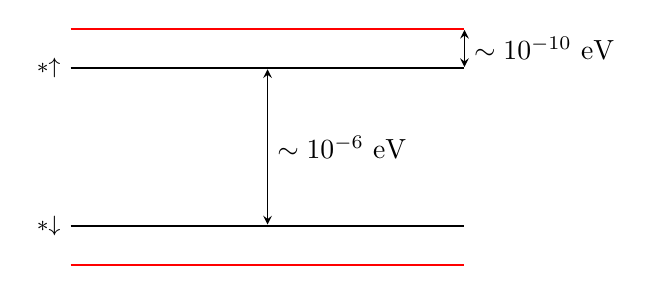
\begin{tikzpicture}
         \draw[thick] (-2.5,1) node[left] {\footnotesize $\ket*{\uparrow}$} -- (2.5,1);
         \draw[thick] (-2.5,-1) node[left] {\footnotesize $\ket*{\downarrow}$} -- (2.5,-1);
         \draw[stealth-stealth, shorten >= 0.4pt, shorten <= 0.4pt] (0,-1) -- (0,1) node[midway,right] {$\sim 10^{-6}$ eV};
         \draw[thick,red] (-2.5,1.5) -- (2.5,1.5);
         \draw[thick,red] (-2.5,-1.5) -- (2.5,-1.5);
         \draw[stealth-stealth, shorten >= 0.4pt, shorten <= 0.4pt] (2.5,1) -- (2.5,1.5) node[midway,right] {$\sim 10^{-10}$ eV};
      \end{tikzpicture}
   \end{figure}
   Inizialmente abbiamo due livelli la cui differenza in energia è di circa $10^{-6} \rm \; eV$. Dopo l'azione della perturbazione, lo stato fondamentale ha avuto una correzione negativa e lo stato eccitato una correzione positiva, entrambi uguali in modulo e pari a circa $10^{-10} \rm \; eV$, per cui il primo si è abbassato e il secondo si è alzato in energia. Tale fatto è generale: ogni volta che agisce una perturbazione, i livelli si allontanano sempre. Ciò è collegato al teorema di incrocio dei livelli, il quale afferma che due livelli non si incrociano mai.
\end{soluzione}

\newpage
\setcounter{equation}{0}

\begin{esercizio}
   Given a proton that scatters on the potential
   \begin{equation*}
      V(r)
      =V_0 \frac{e^{-\alpha r}}{\alpha r}
   \end{equation*}
   with $\alpha=2 \; \rm fm^{-1}$,
   \begin{enumerate}[label=\alph*), leftmargin=0.6cm]
      \item Calculate the phase shift for $\ell=0$ and $\ell=1$ at first order of the Born approximation in the low energy limit and the corresponding total cross section when including both $\ell=0$ and $\ell=1$.
      \item Calculate at what beam energy (in MeV) the cross section associated to $\ell=1$ is equal to $1/10$ of the one associated to $\ell=0$.
      \item If $V_0=20 \rm \; MeV$ is the Born Approximation valid in the low energy limit? Explain your answer.
   \end{enumerate}
   Hint:
   \begin{equation*}
      \int_{0}^{+\infty} \dd{r} r^n e^{-r/r_0}
      =n! \, r_0^{n+1}
   \end{equation*}
\end{esercizio}
\begin{soluzione}
   Osserviamo innanzitutto che il potenziale del problema in esame è un potenziale di Yukawa avente range $R_V$ dato da
   \begin{equation*}
      R_V
      =\frac{1}{\alpha}
      =0.5 \rm \; fm
   \end{equation*}
   Svolgiamo il punto a). Poiché il testo ci fornisce l'espressione per il potenziale, è conveniente usare la formula integrale per il phase shift, la quale è
   \begin{equation*}
      e^{i \delta_{\ell}} \sin{(\delta_{\ell})}
      =-\frac{2 m}{\hbar^2} k \int_{0}^{+\infty} \dd{r} r j_{\ell}(k r) V(r) u_{\ell}(kr)
   \end{equation*}
      Il testo ci dice inoltre di utilizzare l'approssimazione di Born, la quale viene utilizzata quando il potenziale è debole. In conseguenza a ciò, i phase shifts risultano essere piccoli e dunque è possibile usare le approssimazioni $e^{i \delta_{\ell}} \sin{(\delta_{\ell})} \approx \delta_{\ell}$ e $u_{\ell}(kr)=r j_{\ell}(k r)$, per cui possiamo scrivere
   \begin{equation*}
      \delta_{\ell}
      \simeq -\frac{2 m}{\hbar^2} k \int_{0}^{+\infty} \dd{r} r^2 j^2_{\ell}(k r) V(r)
   \end{equation*}
   Poiché siamo nel limite di basse energie, cioè nel limite in cui $k R_V \ll 1$, le funzioni $j_{\ell}$ seguono l'andamento
   \begin{equation*}
      j_{\ell}(kr)
      \simeq \frac{(kr)^{\ell}}{(2 \ell + 1)!!}
   \end{equation*}
   e dunque avremo
   \begin{equation*}
      \delta_{\ell}
      \simeq -\frac{2 m}{\hbar^2} \frac{k^{2 \ell + 1}}{\bigl[ (2 \ell + 1)!! \bigr]^2} \int_{0}^{+\infty} \dd{r} r^{2 \ell + 2} V(r)
   \end{equation*}
   e sostituendo il potenziale fornito si ottiene
   \begin{equation*}
      \delta_{\ell}
      \simeq -\frac{2 m V_0}{\alpha \hbar} \frac{k^{2 \ell + 1}}{\bigl[ (2 \ell + 1)!! \bigr]^2} \int_{0}^{+\infty} \dd{r} r^{2 \ell + 1} e^{-\alpha r}
   \end{equation*}
   Sfruttando il suggerimento fornito dal testo abbiamo che
   \begin{equation*}
      \int_{0}^{+\infty} \dd{r} r^{2 \ell + 1} e^{-\alpha r}
      =\frac{(2 \ell + 1)!}{\alpha^{2 \ell + 2}}
   \end{equation*}
   e dunque
   \begin{equation*}
      \delta_{\ell}
      \simeq -\frac{2 m V_0}{\hbar^2} \frac{1}{\alpha^2} \frac{(2 \ell + 1)!}{\bigl[ (2 \ell + 1)!! \bigr]^2} \qty( \frac{k}{\alpha} )^{2 \ell + 1}
   \end{equation*}
   Osserviamo che in generale l'$\ell$-esimo phase shift deve dipendere da $(kR_V)^{2 \ell + 1}$. Avendo trovato tale dipendenza, abbiamo conferma che quanto fatto finora è corretto.\\
   Calcoliamo i phase shifts per $\ell=0$ e $\ell=1$:
   \begin{equation*}
      \begin{split}
         \delta_0
         & =-\frac{2 m V_0}{\hbar^2} \frac{1}{\alpha^2} \frac{1}{1} \qty( \frac{k}{\alpha} )^{1}
         =-\frac{2 m V_0}{\hbar^2 \alpha^3} k
         \\[0.3cm]
         \delta_1
         & =-\frac{2 m V_0}{\hbar^2} \frac{1}{\alpha^2} \frac{6}{9} \qty( \frac{k}{\alpha} )^{3}
         =-\frac{4 m V_0}{3 \hbar^2 \alpha^5} k^3
      \end{split}
   \end{equation*}
   A questo punto possiamo calcolare la sezione d'urto. Considerando soltanto questi due contributi, essa sarà data da
   \begin{equation*}
      \sigma
      =\frac{4\pi}{k^2} \sum_{\ell=0}^{1} (2 \ell + 1) \delta_{\ell}^2
      =\frac{4\pi}{k^2} \bigl[ \delta_0^2 + 3\delta_1^2 \bigr]
      =\frac{4\pi}{k^2} \qty[ \qty( \frac{2 m V_0}{\hbar^2 \alpha^3} k )^2 + 3 \qty( \frac{4 m V_0}{3 \hbar^2 \alpha^5} k^3 )^2 ]
   \end{equation*}
   Passiamo al quesito b). Per prima cosa calcoliamo le sezioni d'urto relative ai singoli contributi:
   \begin{equation*}
      \sigma_0
      =\frac{4 \pi}{k^2} \qty( \frac{2 m V_0 k}{\hbar^2 \alpha^3} )^2
      \qq{,}
      \sigma_1
      =\frac{4 \pi}{k^2} \qty( \frac{4 m V_0 k^3}{\sqrt{3} \hbar^2 \alpha^5} )^2
   \end{equation*}
   Imponiamo adesso la condizione
   \begin{equation*}
      \sigma_1
      =\frac{1}{10} \sigma_0
   \end{equation*}
   che esplicitando ci dà, dopo aver semplificato,
   \begin{equation*}
      \frac{4}{3} \frac{k^4}{\alpha^4}
      =\frac{1}{10}
   \end{equation*}
   risolvendo rispetto a $k^2$ si ha
   \begin{equation*}
      k^2
      =\frac{\sqrt{3}}{2\sqrt{10}} \alpha^2
      =\rm \frac{\sqrt{3}}{2\sqrt{10}} \, 4 \; fm^{-2}
   \end{equation*}
   a cui corrisponde un'energia
   \begin{equation*}
      E
      =\frac{\hbar^2 k^2}{2 m}
      =\frac{(\hbar c)^2 k^2}{2 m c^2}
      =\rm \frac{4 \cdot 10^2 \; MeV^2 \, fm^2 \cdot 4\sqrt{3} \; fm^{-2}}{2 \cdot 10^3 \; MeV \cdot 2\sqrt{10}}
      =\rm 4\sqrt{10} \; MeV
      \simeq \rm 22.23 \; MeV
   \end{equation*}
   Svolgiamo infine il punto c). Verifichiamo innanzitutto di trovarci nel limite delle basse energie. In corrispondenza del valore di $k$ trovato nel punto b), si ha che
   \begin{equation*}
      k R_V
      =k \frac{1}{\alpha}
      =\qty( \frac{\sqrt{3}}{2\sqrt{10}} )^{\frac{1}{2}} \alpha \frac{1}{\alpha}
      =\qty( \frac{\sqrt{3}}{2\sqrt{10}} )^{\frac{1}{2}}
      \approx 0.52 < 1
   \end{equation*}
   Seppur tale quantità non molto minore di 1, possiamo comunque considerarci nel limite di basse energie.\\
   Passiamo a verificare la validità dell'approssimazione di Born. Nel caso di basse energie, la condizione da soddisfare è
   \begin{equation*}
      \frac{2 m V_0}{\hbar^2} R_V
      \ll 1
   \end{equation*}
   che sostituendo i valori numerici ci dà
   \begin{equation*}
      \frac{2 mc^2 V_0}{(\hbar c)^2} \frac{1}{\alpha}
      =\rm \frac{2 \cdot 10^3 \; MeV \cdot 20 \; MeV}{4 \cdot 10^4 \; MeV^2 \, fm^2} \frac{1}{2 \; fm^{-1}}
      =0.5 < 1
   \end{equation*}
   dunque l'approssimazione di Born è valida.
\end{soluzione}

\newpage
\setcounter{equation}{0}

\begin{esercizio}
   An electron movers in a one-dimensional square well potential
   \begin{equation*}
      V(x)=
      \begin{cases}
         0 & \text{if } |x|<L\\
         \infty & \text{if } |x|>L
      \end{cases}
   \end{equation*}
   And is perturbed by an electric field.
   \begin{enumerate}[label=\alph*), leftmargin=0.6cm]
      \item Consider a weak uniform electric field of strenght $\mathcal{E}_0$ acting on the electron as the figure ($V(x)= e \mathcal{E}_0 x$).
      \begin{figure}[H]
         \centering
         \begin{tikzpicture}[scale=0.8]
            \fill[pattern=north east lines] (-5,-2.5) rectangle (-3,2.5);
            \fill[pattern=north east lines] (5,-2.5) rectangle (3,2.5);
            \draw[->] (-5,0) -- (5.3,0) node[right] {$x$};
            \draw[->] (0,-2.5) -- (0,2.5) node[above] {$V(x)$};
            \draw[thick, cyan!60!black] (-3,-2) -- (3,2);
            \node[below right] at (-3,0) {$-L$};
            \node[below left] at (3,0) {$L$};
         \end{tikzpicture}
      \end{figure}
      Use WKB approximation to calculate the energy levels, and find the minimum value of $\mathcal{E}_0$ to have at least one negative energy level for $L=3 \; \rm nm$.
      \item Consider now the case of a time-dependent electric field
      \begin{equation*}
         \mathcal{E}(t)
         =\mathcal{E}_0 e^{-t/\tau}
      \end{equation*}
      for $t>0$. Calculate the transition probability from the ground state to the first excited state in first-order time-dependent perturbation theory for times $t \gg \tau$ and the value of $\mathcal{E}_0$ and $L$ from a) and $\tau=10^{-14} \; \rm s$.
   \end{enumerate}
   Hint:
   \begin{equation*}
      \int_{-L}^{L} \dd{x} \sin{ \qty( \frac{\pi x}{L} ) } \sin{ \qty( \frac{\pi x}{L} ) }
      =\frac{32}{9} \frac{\pi^2}{L^2}
   \end{equation*}
\end{esercizio}
\begin{soluzione}
  Svolgiamo il punto a). Il testo ci chiede di trovare un valore di $\mathcal{E}_0$ tale da avere almeno un livello ad energia negativa, dunque in base all'andamento del potenziale dobbiamo applicare le formule dell'approssimazione WKB nella regione tra $x=-L$ e $x=0$. In tal caso, la condizione che serve per calcolare i livelli di energia è quella nel caso di una buca con una sola parete, cioè
   \begin{equation*}
      \int_{x_1}^{x_2} \dd{x} \sqrt{2m \bigl[ E - V(x) \bigr]}
      =\qty( n - \frac{1}{4} )\pi \hbar
      \qq{,}
      n=1,2,\ldots
   \end{equation*}
   con $x_1$ e $x_2$ i classical turning points. In particolare, abbiamo che $x_1=-L$, mentre $x_2$ sarà un certo punto per cui $V(x_2)=E$. Esplicitando anche il potenziale, avremo che
   \begin{equation}
      \int_{-L}^{x_2} \dd{x} \sqrt{2m ( E - e \mathcal{E}_0 x )}
      =\qty( n - \frac{1}{4} )\pi \hbar
      \qq{,}
      n=1,2,\ldots
      \label{eq:condizione_WKB_potenziale_lineare_con_una_barriera}
   \end{equation}
   Per risolvere questo integrale adoperiamo la sostituzione
   \begin{equation*}
      z=2m ( E - e \mathcal{E}_0 x )
      \implies
      \dd{z}
      =-2m e \mathcal{E}_0 \dd{x}
   \end{equation*}
   e dunque riscriviamo l'integrale come
   \begin{equation*}
      -\frac{1}{2 m e \mathcal{E}_0} \int_{2m(E + e \mathcal{E}_0 L)}^{0} \dd{z} \sqrt{z}
      =-\frac{1}{2 m e \mathcal{E}_0} \qty[ \frac{2}{3} z^{\frac{3}{2}} ]_{2m(E + e \mathcal{E}_0 L)}^{0}
      =\frac{1}{3 m e \mathcal{E}_0} \bigl[ 2m(E + e \mathcal{E}_0 L) \bigr]^{\frac{3}{2}}
   \end{equation*}
   Inserendo tale risultato nella \eqref{eq:condizione_WKB_potenziale_lineare_con_una_barriera} otteniamo
   \begin{equation*}
      2m(E + e \mathcal{E}_0 L)
      =\qty[ 3 m e \mathcal{E}_0 \pi \hbar \qty( n - \frac{1}{4} ) ]^{\frac{2}{3}}
   \end{equation*}
   da cui segue i livelli energetici sono dati da
   \begin{equation*}
      E_n
      =-e \mathcal{E}_0 L + \frac{1}{2m} \qty[ 3 m e \mathcal{E}_0 \pi \hbar \qty( n - \frac{1}{4} ) ]^{\frac{2}{3}}
      \qq{,}
      n=1,2,\ldots
   \end{equation*}
   A noi interessa trovare il minimo valore di $\mathcal{E}_0$ tale che esista almeno un livello ad energia negativa, dunque poniamo $n=1$ e risolviamo l'equazione
   \begin{equation*}
      E_1
      =- e \mathcal{E}_0 L + \frac{1}{2m} \qty( 3 m e \mathcal{E}_0 \pi \hbar \frac{3}{4} )^{\frac{2}{3}}
      \leq 0
   \end{equation*}
   da cui
   \begin{gather*}
      e \mathcal{E}_0 L
      \geq \frac{1}{2m} \qty( \frac{9}{4} m e \mathcal{E}_0 \pi \hbar )^{\frac{2}{3}}
      \\
      \implies
      e^3 \mathcal{E}_0^3 L^3
      \geq \qty( \frac{1}{2m} )^3 \qty( \frac{9}{4} m e \pi \hbar )^{2} \mathcal{E}_0^2
      \\
      \implies
      e \mathcal{E}_0
      \geq \frac{81}{128} \frac{\pi^2 \hbar^2}{m L^3}
   \end{gather*}
   ovvero, sostituendo i valori numerici,
   \begin{equation*}
      e \mathcal{E}_0
      \geq \frac{81}{128} \frac{\pi^2 (\hbar c)^2}{m c^2 L^3}
      =\frac{81}{128} \frac{\pi^2 \cdot 4 \cdot 10^4 \; \rm eV^2 \, \rm nm^2}{0.5 \cdot 10^6 \; \rm eV \cdot 27 \; \rm nm^3}
      = 1.87 \; \rm eV/\rm nm
   \end{equation*}
   dunque il valore cercato è $\mathcal{E}_0 \approx 2 \cdot 10^7 \; \rm V/m$.\\
   Passiamo al punto b). Dobbiamo trovare la probabilità di transizione dal ground state al primo stato eccitato\footnote{\E da notare che i livelli da considerare sono quelli della buca quadra senza la presenza del campo elettrico. Ciò è confermato anche dal fatto che il testo dice di considerare un nuovo caso.}. In questo caso, visto che la buca si estende da $-L$ ad $L$, le funzioni d'onda sono date da\footnote{Si presti attenzione al fatto che in questo caso le funzioni d'onda hanno parità rispetto alla buca che è opposta rispetto a quella di $n$, per cui saranno dispari per $n$ pari e pari per $n$ dispari.}
   \begin{equation*}
      \psi_n(x)
      =
      \begin{cases}
         \displaystyle \sqrt{\frac{1}{L}}\cos{ \qty( \frac{n \pi x}{2L} ) } & \text{per $n$ dispari}\\[0.3cm]
         \displaystyle \sqrt{\frac{1}{L}}\sin{ \qty( \frac{n \pi x}{2L} ) } & \text{per $n$ pari}
      \end{cases}
   \end{equation*}
   mentre le energie sono date da\footnote{Da notare che il fattore $8$ deriva dal fatto che la larghezza della buca è $2L$.}
   \begin{equation*}
      E_n
      =\frac{\hbar^2 \pi^2}{8 m L^2} n^2
      \qq{,}
      n=1,2,\ldots
   \end{equation*}
   Avendo un campo elettrico, il potenziale perturbativo sarà dato da
   \begin{equation*}
      V'(t)
      =e \mathcal{E}_0 x e^{-t/\tau}
   \end{equation*}
   pertanto l'ampiezza di transizione dal ground state al primo stato eccitato sarà data da
   \begin{equation*}
      c_{1 \to 2}
      =-\frac{i}{\hbar} \int_{0}^{t} e^{i \omega_{21} t'} V_{2,1}(t') \dd{t'}
   \end{equation*}
   dove
   \begin{equation*}
      \omega_{21}
      =\frac{E_2 - E_1}{\hbar}
      =\frac{3 \pi^2 \hbar^2}{8 m L^2}
   \end{equation*}
   e
   \begin{gather*}
      V_{2,1}(t)
      =\mel*{\psi_2}{V'}{\psi_1}
      =e \mathcal{E}_0 e^{-t/\tau} \mel*{\psi_2}{x}{\psi_1}
      \\
      =e \mathcal{E}_0 e^{-t/\tau} \frac{1}{L} \int_{-L}^{L} \dd{x} x \sin{ \qty( \frac{\pi x}{L} ) } \cos{ \qty( \frac{\pi x}{2L} ) }
      =e \mathcal{E}_0 e^{-t/\tau} \frac{32 L}{9 \pi^2}
   \end{gather*}
   avendo sfruttato il suggerimento fornito dal testo. Inserendo le espressioni trovate, otteniamo
   \begin{equation*}
      c_{1 \to 2}
      =-\frac{i}{\hbar} e \mathcal{E}_0 \frac{32 L}{9 \pi^2} \int_{0}^{t} e^{i \qty( \omega_{21} - \frac{1}{\tau}) t'} \dd{t'}
      =-\frac{i}{\hbar} e \mathcal{E}_0 \frac{32 L}{9 \pi^2} \frac{e^{i \qty( \omega_{21} - \frac{1}{\tau}) t} - 1}{i \qty( \omega_{21} - \frac{1}{\tau})}
   \end{equation*}
   Se adesso imponiamo la condizione $t \gg \tau$, otteniamo\footnote{In questo modo stiamo ponendo $e^{i \frac{t}{\tau}}\approx 1$.}
   \begin{equation*}
      c_{1 \to 2}
      \approx -\frac{i}{\hbar} e \mathcal{E}_0 \frac{32 L}{9 \pi^2} \frac{e^{i \omega_{21} t} \tau}{i \omega_{21} \tau - 1}
   \end{equation*}
   e dunque la probabilità sarà
   \begin{equation*}
      P_{1 \to 2}
      =|c_{1 \to 2}|^2
      =\qty( \frac{32 e \mathcal{E}_0 L}{9 \pi^2 \hbar} )^2 \frac{\tau^2}{\omega_{21}^2 \tau^2 + 1}
   \end{equation*}
   Osserviamo adesso che
   \begin{equation*}
      \omega_{21}
      =\frac{3 \pi^2 c \hbar c}{8 mc^2 L^2}
      =\frac{3 \pi^2 \cdot 3 \cdot 10^{17} \; \rm nm \, s^{-1} \cdot 2 \cdot 10^2 \; eV^2 \, nm^2}{8 \cdot 0.5 \cdot 10^6 \; \rm eV \cdot 9 \; \rm nm^2}
      \simeq 0.5 \cdot 10^{14} \; \rm s^{-1}
   \end{equation*}
   per cui $\omega_{2,1}\tau=0.5$. Inserendo tale risultato nella probabilità e sostituendo gli altri valori, abbiamo
   \begin{equation*}
      P_{1 \to 2}
      =\rm \qty( \frac{32 \cdot 2 \; eV \, nm^{-1} \cdot 3 \; nm}{9 \pi^2 \cdot 6.6 \cdot 10^{-16} \; eV \, s} )^2 \, \frac{10^{-28} \; s^{-2}}{0.5^2 + 1}
      =0.08 \ll 1
   \end{equation*}
\end{soluzione}

\newpage
\setcounter{equation}{0}